\section{Fotometría}

Para este trabajo se realizó una campaña de observación durante los últimos
meses del 2022, con la finalidad de observar el sistema durante una fase orbital
completa. Las fechas y duraciones de cada día de observación se encuentra en la
\reftable{observationSchedules}. Durante varias de estas noches de observación
las condiciones del sitio fueron menos que ideal; tanto las condiciones
meteorológicas como contratiempos causados por el equipo en si causaron
interrupciones en la medición del brillo del sistema. Esto es esperado en un
observatorio en proceso de desarrollo; a pesar de los problemas técnicos, se
pudieron obtener datos de calidad aceptable. 

% TODO: style table
\begin{table}[!ht]
	\centering
	\begin{tabular}{|l|l|l|l|}
		\hline
		\thead{Fecha} & \thead{HJD Inicio +\textbf{\num{2459000}}} & \thead{Tiempo Expocisiones} & \thead{Duración} \\
		\hline
		2022-10-21 & 874.66 & $114 \cdot 60$ s & 2.59 h \\
		\hline
		2022-10-27 & 880.77 & $93 \cdot 60$ s & 1.86 h \\
		\hline
		2022-11-05 & 889.67 & $98 \cdot 60$ s & 2.02 h \\
		\hline
		2022-11-26 & 910.72 & $56 \cdot 60$ s & 1.55 h \\
		\hline
		2022-12-06 & 920.55 & $243 \cdot 60$ s & 4.90 h \\
		\hline
		2022-12-07 & 921.56 & $163 \cdot 60$ s & 4.20 h \\
		\hline
		2022-12-08 & 922.53 & $188 \cdot 60$ s & 5.57 h \\
		\hline
		2022-12-09 & 923.54 & $119 \cdot 60$ s & 5.33 h \\
		\hline
		2022-12-10 & 924.53 & $122 \cdot 60$ s & 2.20 h \\
		\hline

	\end{tabular}
	\caption{Fechas de observaciones fotométricas desde el OAU.}
	\label{observationSchedules}
\end{table}

\begin{figure}[!ht]
	\centering
	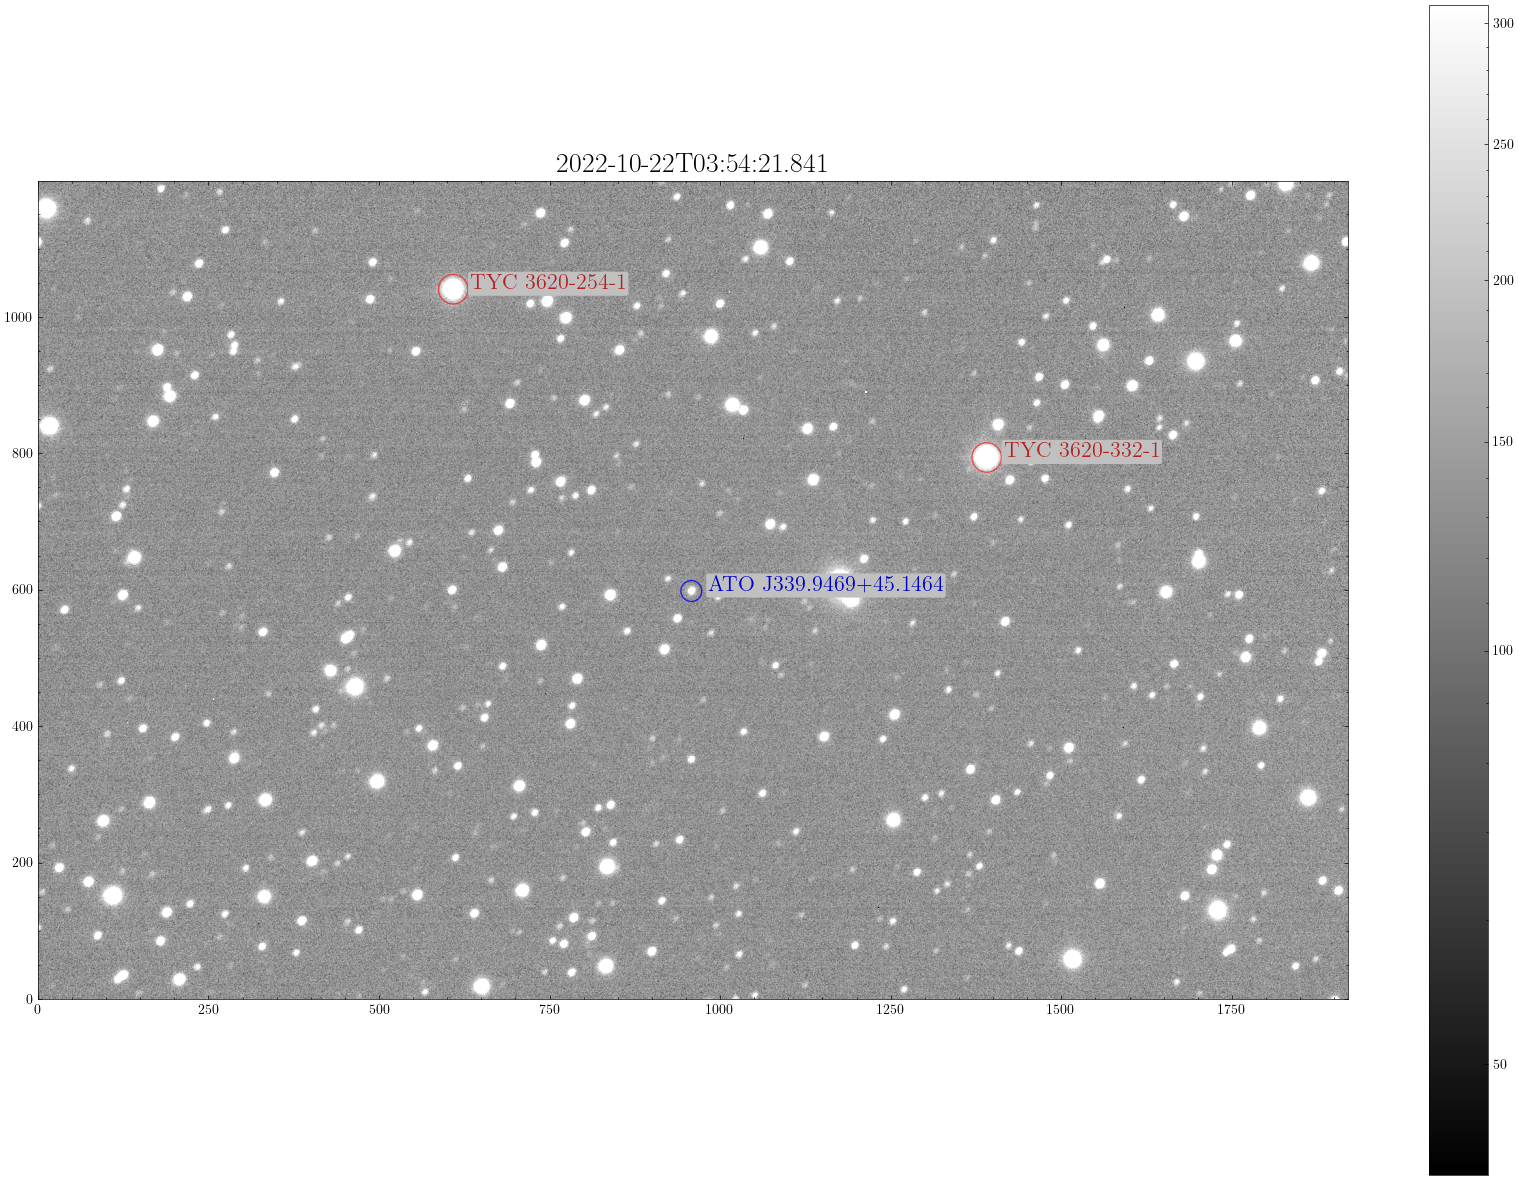
\includegraphics[scale=0.4]{Observaciones/Secciones/Figures/10-22 Sample Image.png}
	\caption{Imagen del campo de \atoObjIdNoSpace, junto a 2 estrellas de comparación usadas en la fotometría diferencial marcadas en anillos rojos.}
	\label{ccdImageField}
\end{figure}

\subsection{Estrellas de Comparación}

Para determinar la magnitud diferencial de un objeto se necesita una estrella de
comparación que yazca dentro del campo de la imagen de ciencias. Una manera de
encontrar estrellas de referencias adecuadas es utilizando el
\href{https://app.aavso.org/vsp/}{Variable Star Plotter} de la \textit{AAVSO};
sin embargo, debido al diminuto campo de visión de nuestras imágenes
(aproximadamente 1' de largo), no se encuentra alguna estrella standard
registrada. Por lo tanto se utilizaron estrellas no variables de la base de
datos de SIMBAD:
\href{http://simbad.cds.unistra.fr/simbad/sim-id?Ident=%406898031&Name=TYC%203620-254-1&submit=submit}{TYC
3620-254-1} y
\href{http://simbad.cds.unistra.fr/simbad/sim-id?Ident=%406898038&Name=TYC%203620-332-1&submit=submit}{TYC
3620-332-1}. Sus posiciones relativo a la estrella objetivo \atoObjId se puede
ver en la figura \ref{ccdImageField}.

\subsection{Procesamiento de Imágenes}

La limpieza de las imágenes incluyó la corrección de bias, darks, y flats por
medio de imágenes de calibración, las cuales fueron tomadas cada noche de
observación. Esta sustracción se realizó utilizando el paquete \code{ccdproc} en
Python, haciendo uso de sus funciones dedicadas al procesamiento de imágenes de
CCD \autocite{ccdproc241}. El código relevante se puede encontrar en el notebook
\href{https://github.com/KnightIV/UANL_MAPTA_Observaciones/blob/main/analisis/iturbide/photometry_clean.ipynb}{\code{photometry\_clean.ipynb}}.
Una vez que las mediciones hayan sido corregidas de errores sistemáticos, fue
necesario trasladar los datos dentro de las imágenes para que \atoObjId quede en
el centro del campo, facilitando la fotometría por apertura. Dentro del mismo
notebook
\href{https://github.com/KnightIV/UANL_MAPTA_Observaciones/blob/main/analisis/iturbide/photometry_clean.ipynb}{\code{photometry\_clean.ipynb}}
se ejecutó una tarea de \textit{plate solving} para cada imagen calibrada; el
proceso de \textit{plate solve}, llevado a cabo utilizando \textit{Astrometry}
\autocite{astrometry}, toma como referencia estrellas dentro del campo de la
imagen, comparando contra una base de datos pre-definida para determinar las
coordenadas físicas que corresponden a una imagen. Esta información va
encapsulada dentro de los metadatos del archivo FITS, conocido como
\textbf{World Coordinate System} (\textbf{WCS}). Una vez que una imagen sea
resuelta se puede proyectar a las coordenadas de otra imagen, efectivamente
\quotes{apilando} el sistema a observar.

\begin{figure}[!ht]
	\centering
	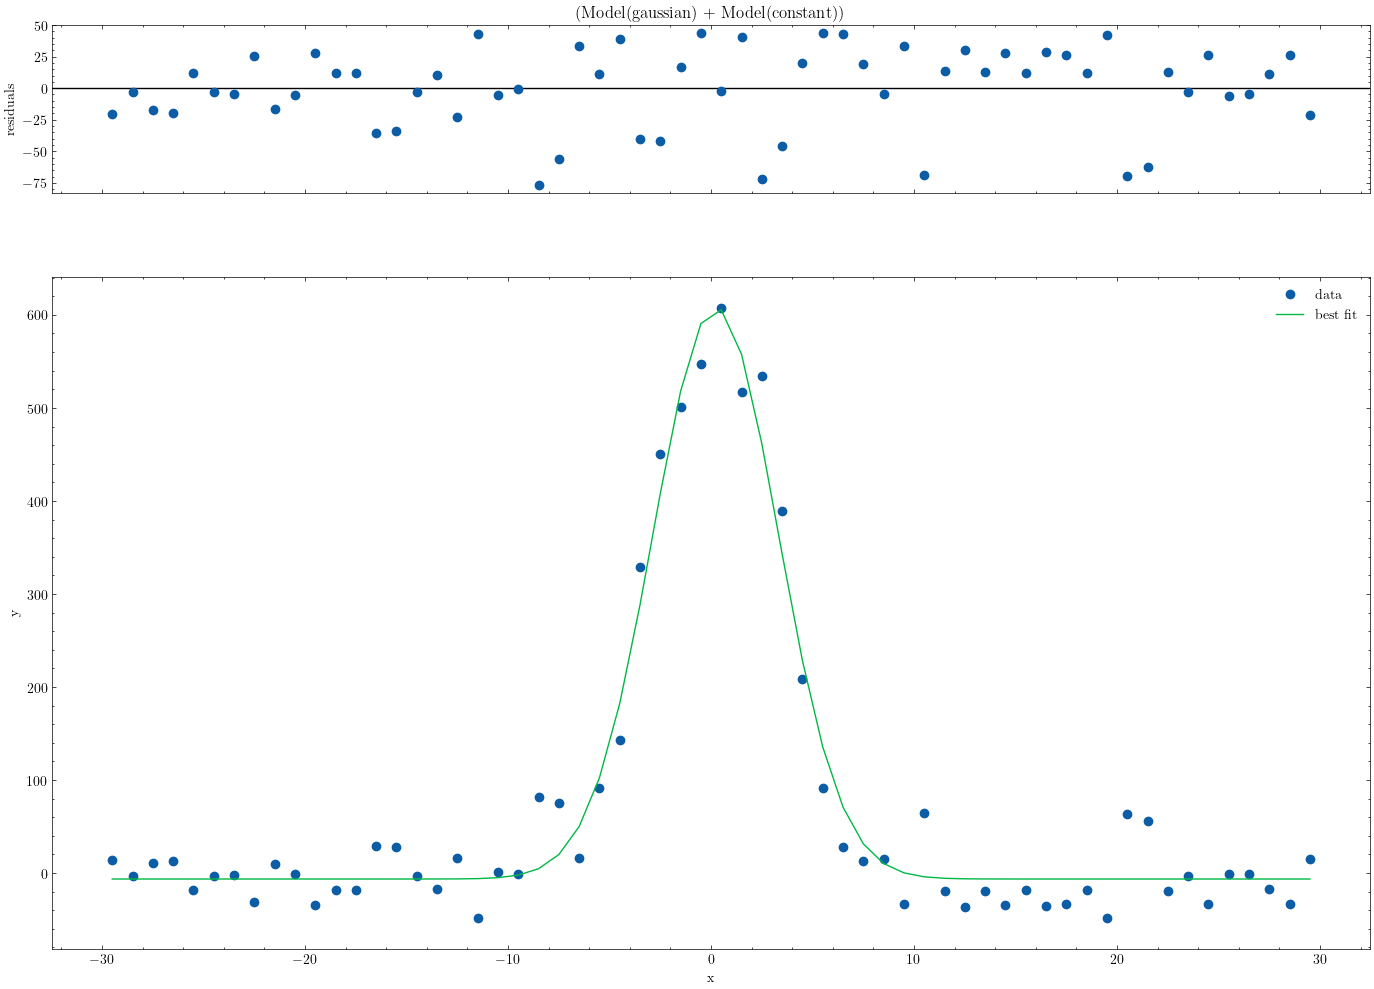
\includegraphics[scale=0.44]{Observaciones/Secciones/Figures/Pixel Radial Profile - Gaussian.png}
	\caption{Perfil Gaussiano de \atoObjId. Esta imagen fue generada en el
	notebook
	\href{https://github.com/KnightIV/UANL_MAPTA_Observaciones/blob/main/analisis/iturbide/iraf/qphot_params_helper.ipynb}{\code{qphot\_params\_helper.ipynb}},
	en donde se toma un corte transversal los pixeles del centro de la imagen
	del sistema. A este perfil radial se hace un ajuste de modelo Gaussiano con
	la finalidad de determinar un tamaño adecuado de aperturas basado en la
	anchura del modelo.}
	\label{pixelGaussProfile}
\end{figure}

Utilizando las imágenes proyectadas se obtuvo el brillo de \atoObjId utilizando
la tarea \code{qphot} de IRAF, dando como resultado magnitudes y flujos
instrumentales del sistema. Para elegir el mejor tamaño de apertura para cada
día se realizó un análisis del comportamiento del brillo de ambas estrellas de
referencia; ya que estas se conocen que son estrellas singulares que carecen de
variabilidad intrínseca esperamos que sus magnitudes a lo largo del tiempo no
muestren cambios significativos. Al mismo tiempo, debido a las condiciones
variables durante cada noche de observación no todas las magnitudes medidas
resultaron útiles debido a una imagen barrida. Para no tener que descartar toda
una noche de observación se implementó un proceso de \textit{sigma clipping}, en
el cual se descartan aquellas observaciones que caen fuera de un rango aceptable
pre-determinado, tomando TYC 3620-332-1 como estrella de referencia. El proceso
completo se encuentra en el código
\href{https://github.com/KnightIV/UANL_MAPTA_Observaciones/blob/main/analisis/iturbide/iraf/qphot_sigma_clip.ipynb}{\code{qphot\_sigma\_clip.ipynb}}.

\begin{figure}[!ht]
	\centering
	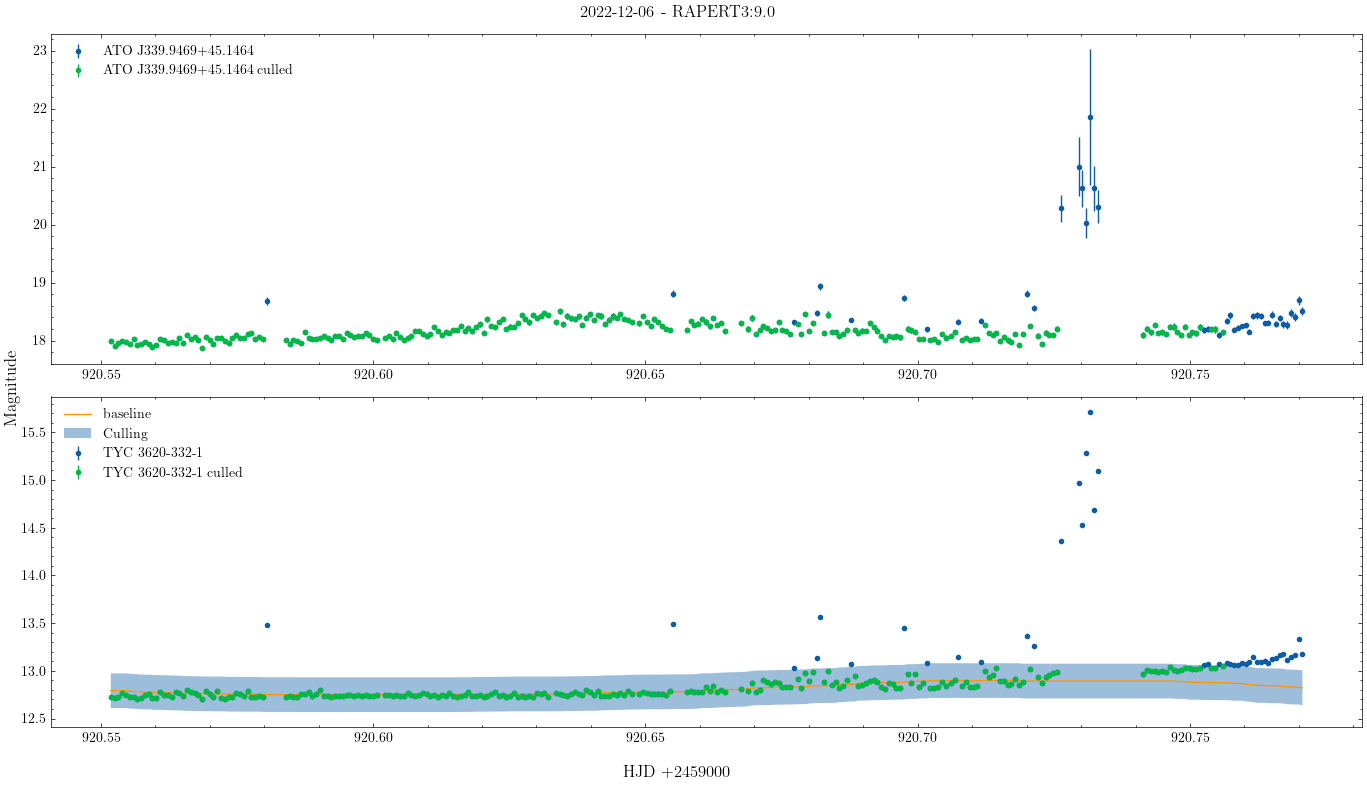
\includegraphics[scale=0.48]{Observaciones/Secciones/Figures/Sigma Clip.png}
	\caption{Resultado del sigma clipping para el 6 de diciembre. Este proceso
		se ejecutó para cada fecha de observación, con el fin de eliminar solo
		los datos más problemáticos. La línea base fue construida usando una
		técnica de media recorrida, para solo descartar aquellos datos cuya
		variación local es significante.}
	\label{sigmaClipSingleDate}
\end{figure}

\subsection{Fotometría Diferencial}
% TODO: upload raw data to GitHub repo and link here
Para obtener una magnitud diferencial de \atoObjId se necesita de una estrella
de referencia cuya magnitud en el visible es conocida y bien estudiada.
\compstarId ha sido observada por varios sondeos, por lo cual se ha medido su
magnitud en el visible de 11.57. Utilizando esta estrella conocida podemos
calcular la magnitud diferencial de \atoObjId con la \refequation{observaciones:fotometriadiferencial:magdiferencialec}. Una gran ventaja de
la fotometría diferencial a comparación de magnitudes absolutas es que llega a
minimizar los efectos causados por obstrucciones del cielo, como nubes
intermitentes o celdas turbulentas en la atmósfera. Los resultados para un día
de observación se encuentra en la \reffigure{differentialMagDec7}, donde se
puede apreciar la variabilidad de \atoObjId comparado con ambas estrellas de
referencia. Este proceso se repite para cada noche de observación, al final
obteniendo una curva de luz del sistema visto en la
\reffigure{iturbideAtoLightCurve}. El código completo se encuentra en
\href{https://github.com/KnightIV/UANL_MAPTA_Observaciones/blob/main/analisis/iturbide/iraf/qphot_sigma_clip.ipynb}{\code{qphot\_sigma\_clip.ipynb}}.

% Aquí se calcula el
% error en las magnitudes instrumentales con la diferencia entre la magnitud
% medida de TYC 3620-332-1 y su magnitud en el visible reportada en SIMBAD
\begin{eqfloat}[!ht]
	\begin{equation} \label{observaciones:fotometriadiferencial:magdiferencialec}
		\begin{split}
			& E_{\mathrm{inst}} = V_{\mathrm{\compstarIdNoSpace}} - V_{\mathrm{\compstarIdNoSpace}, \mathrm{inst}} \\
			& V_{\mathrm{\atoObjId}} = V_{\mathrm{\atoObjId}, \mathrm{inst}} - E_{\mathrm{inst}}
		\end{split}
	\end{equation}
	\caption{Ecuación para obtener la magnitud diferencial de \atoObjIdNoSpace.
	El primer paso es calcular el error en las magnitudes diferenciales medidas,
	$E_{\mathrm{inst}}$ utilizando la magnitud conocida de nuestra estrella de
	comparación, \compstarIdNoSpace, $ V_{\mathrm{\compstarIdNoSpace}}$ y
	restando la magnitud instrumental medida de las imágenes de observación. Una
	vez obtenido el error este se resta de la magnitud instrumental de
	\atoObjIdNoSpace, $V_{\mathrm{\atoObjId}, \mathrm{inst}}$, obteniendo su
	magnitud diferencial en el visible $V_{\mathrm{\atoObjId}}$.}
\end{eqfloat}
	
\begin{figure}[!ht] 
	\centering
	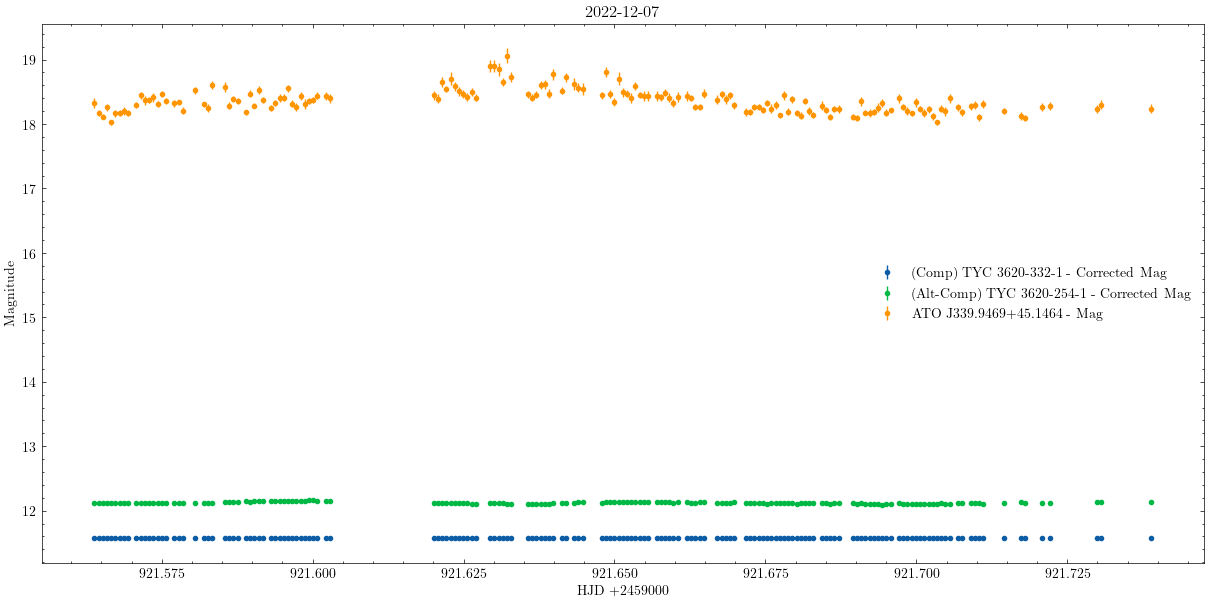
\includegraphics[scale=0.5]{Observaciones/Secciones/Figures/Differential Magnitude 12-07.png}
	\caption{Magnitud diferencial para \atoObjId junto a las magnitudes de TYC
	3620-332-1 y TYC 3620-254-1. Esta segunda estrella fue utilizada como
	estrella de campo, para corroborar que la resta descrita en la ecuación
	\ref{observaciones:fotometriadiferencial:magdiferencialec} adecuadamente
	eliminó los errores sistemáticos en otra estrella de referencia.}
	\label{differentialMagDec7}
\end{figure}

\begin{figure}[!ht]
	\centering
	\xincludegraphics[scale=0.4, label=\textbf{(a)}, labelbox=true, pos=nw, fontsize=\large]{Observaciones/Secciones/Figures/Full LC.png}
	\xincludegraphics[scale=0.4, label=\textbf{(b)}, labelbox=true, pos=nw, fontsize=\large]{Observaciones/Secciones/Figures/Hour Sync LC.png}
	\caption{Magnitud diferencial de \atoObjIdNoSpace. Ambas gráficas muestran
	los errores de medición, las cuales fueron más altas de lo ideal debido a
	las condiciones del sitio. \textbf{a)} Curva de luz completa, con cada día
	de observación. \textbf{b)} Curva de luz segmentada por día. Aquí se logra
	apreciar la cadencia de observación, viendo como cada día se logra observar
	una fase diferente del sistema.}
	\label{iturbideAtoLightCurve}
\end{figure}